%!TEX root = ../summary.tex

\section{From Source Code to Physical Deployment}

\subsection{Version Control Systems}
Versioning aims to control an manage all artifacts used and created in a process.
VCSes can be differentiated between local, centralized and distributed VCSes.
Local ones are kept only on the local systems where the artifacts are developed.
Centralized VCSes have a central server that holds the code base and single clients have only a single version of the artifacts available.
Distributed VCSes have different versions locally as well as on a central repository.

\subsubsection{SVN (central) vs Git (distributed)}
SVN stores information as a list of file-based changes.
Git on the other hand handles the data more like a set of snapshots of a miniature file system.
Every commit is a picture taken of what all files look like at that moment and pointers to these snapshots are stored.

\subsubsection{Git}
\paragraph{File States}
In Git, a file can have three different stages.
In the modified state the file has changes that are not yet committed to the local database.
In the staged state the file then has been marked to go into the next commit and in the committed state the data is safely stored in the local database.
In that state the data can be pushed to the remote repository.

\paragraph{Commands}
\begin{figure}[H]
  \centering
  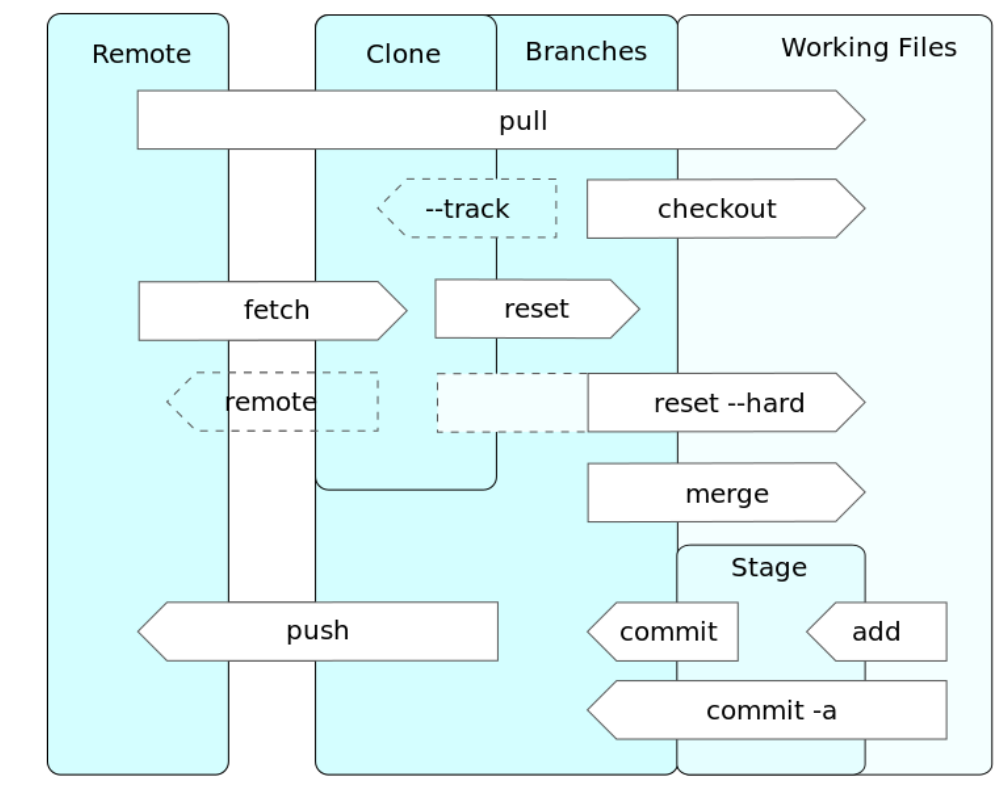
\includegraphics[width=.8\textwidth]{images/git_commands.png}
  \caption{Git Commands}
\end{figure}

\paragraph{Branching}
Git keeps snapshots of the commits named by hashes of the local files.
Branches are pointers to these commits.
The HEAD pointer points to the current local commit, the default branch is called master and adding a branch means adding a named pointer to a commit.

\subsection{Continuous Integration}
\begin{figure}[h]
  \centering
  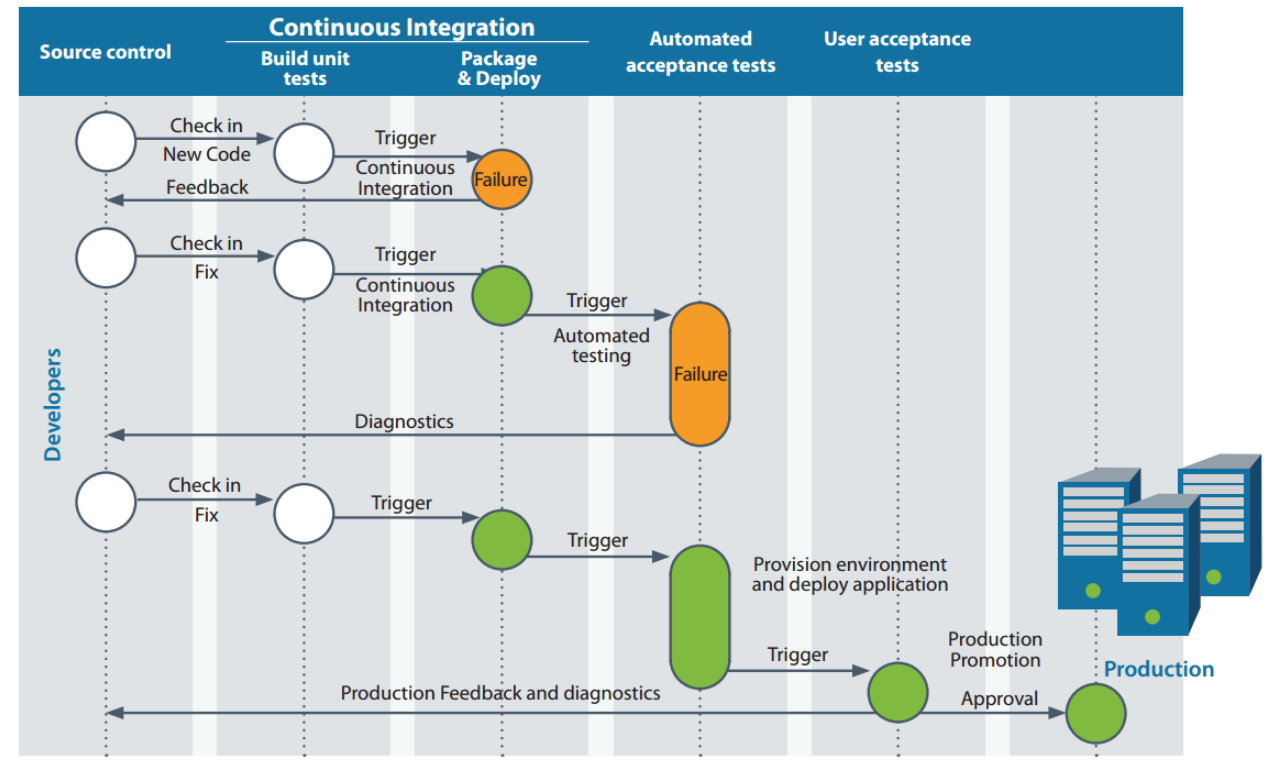
\includegraphics[width=.8\textwidth]{images/continuous_integration.png}
  \caption{Continuous Integration}\label{fig:continuous_integration}
\end{figure}
A development process (c.f.\ Figure~\ref{fig:continuous_integration}) with continuous integrations maintains a single source repository with an automated build and tests.
Every commit triggers a this automated procedures for what it is important to keep the build process fast.
Test should be executed in a clone of the production environment.
The automated build process makes it easy for everyone to get the latest executables and makes the result visible to everyone.
In the end, even the deployment can be automated potentially.\\

\textbf{Pros}
\begin{itemize}[topsep=0pt, noitemsep]
  \item Reducing risk
  \item Integrated quality assurance
  \item Reports and feedback on the health of the code base
  \item Availability of a stable release
  \item Everyone commits to the main branch every day which results in modular, less complex code
\end{itemize}

\subsection{Continuous Deployment}
Continuous deployment means that every change goes through the pipeline and automatically gets put into production, resulting in many production deployments every day.
For continuous deployment continuous delivery is necessary.
This is a software engineering approach in which teams keep producing valuable software in short cycles and ensure that the software can be reliably released at any time.\\

A deployment pipeline is essential for automating the deployment process.
It represents an automated manifestation of the process of getting software from version control into the hands of the users.
It builds binaries deploys them the same way in every environment after some ``smoke-tests''.
If it fails at any point, the deployment process is stopped.

\paragraph{Deployment-automation Patterns}
\begin{figure}[H]
  \centering
  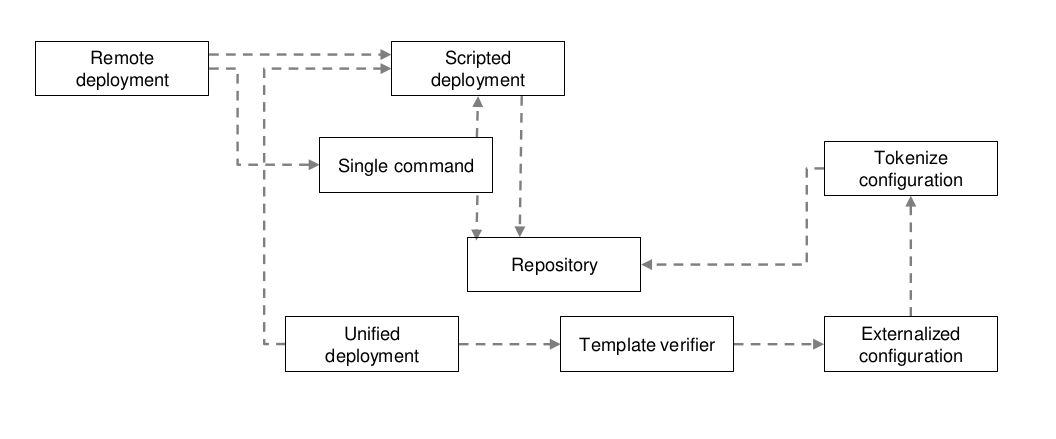
\includegraphics[width=.8\textwidth]{images/deployment_automation_patterns.png}
  \caption{Deployment-automation Patterns}
\end{figure}
\begin{description}
  \item[Repository] All files are committed to version-control repository — in the deployment context, all of the configuration files and tools.
  \item[Scripted deployment] All deployment processes are written in a script.
  \item[Single command] Deployers, or headless processes, can type a single command to generate working software for users.
  \item[Externailzed configuration] All variable values are externalized from the application configuration into build-time properties.
  \item[Tokenize configuration] Token values are entered into configuration files and then replaced during the Scripted Deployment based on Externalized Configuration properties checked into Repository.
  \item[Template verifier] Create a single template file that all target environment properties are based on.
  \item[Unified deployment] Create a single deployment script capable of running on different platforms and target environments.
  \item[Remote deployment] Use a centralized machine or cluster to deploy software to multiple target environments.
\end{description}

\paragraph{Blue Green Deployment}
In blue green deployment, two different production environments are maintained.
In the start the blue one is live.
For a new release, perform a final stage of testing in the green environment and once the software is working, switch to green.

\subsection{Virtual Machines and Containers}
\paragraph{Virtualization}
Virtualization is a combination of software and hardware engineering that creates Virtual Machines (VMs) - an abstraction of the computer hardware that allows a single machine to act as if it where many machines.
This enables the current model of data centers where many virtual machines run on one machine.

\paragraph{Containers}
Containers apply virtualization at the operating system level instead of the hardware level (c.f.\ Figure~\ref{fig:container_vs_virtual_machines}).
This makes containers smaller than hypervisor guests but does not allow running different kernels and has a more loosely approach to isolation and security.\\
\begin{figure}[h]
  \centering
  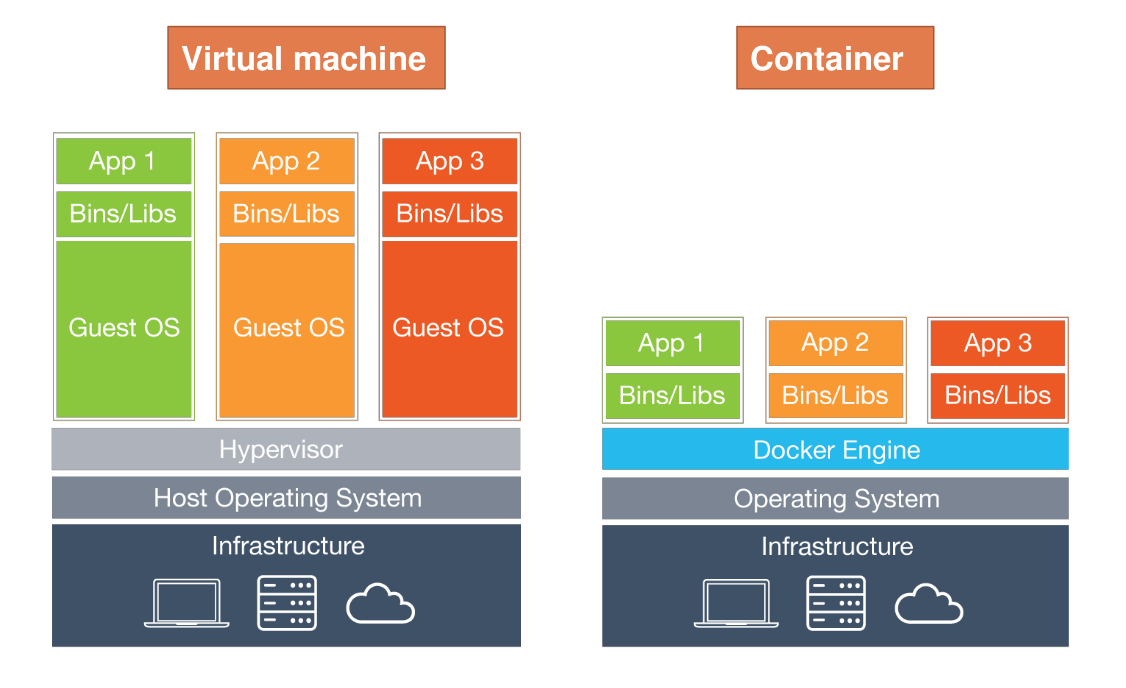
\includegraphics[width=.8\textwidth]{images/container_vs_virtual_machines.png}
  \caption{Virtual Machines vs Application Containers}\label{fig:container_vs_virtual_machines}
\end{figure}

The most popular system for container virtualization is Docker.
Its system is depicted in Figure~\ref{fig:docker}.
\begin{figure}[h]
  \centering
  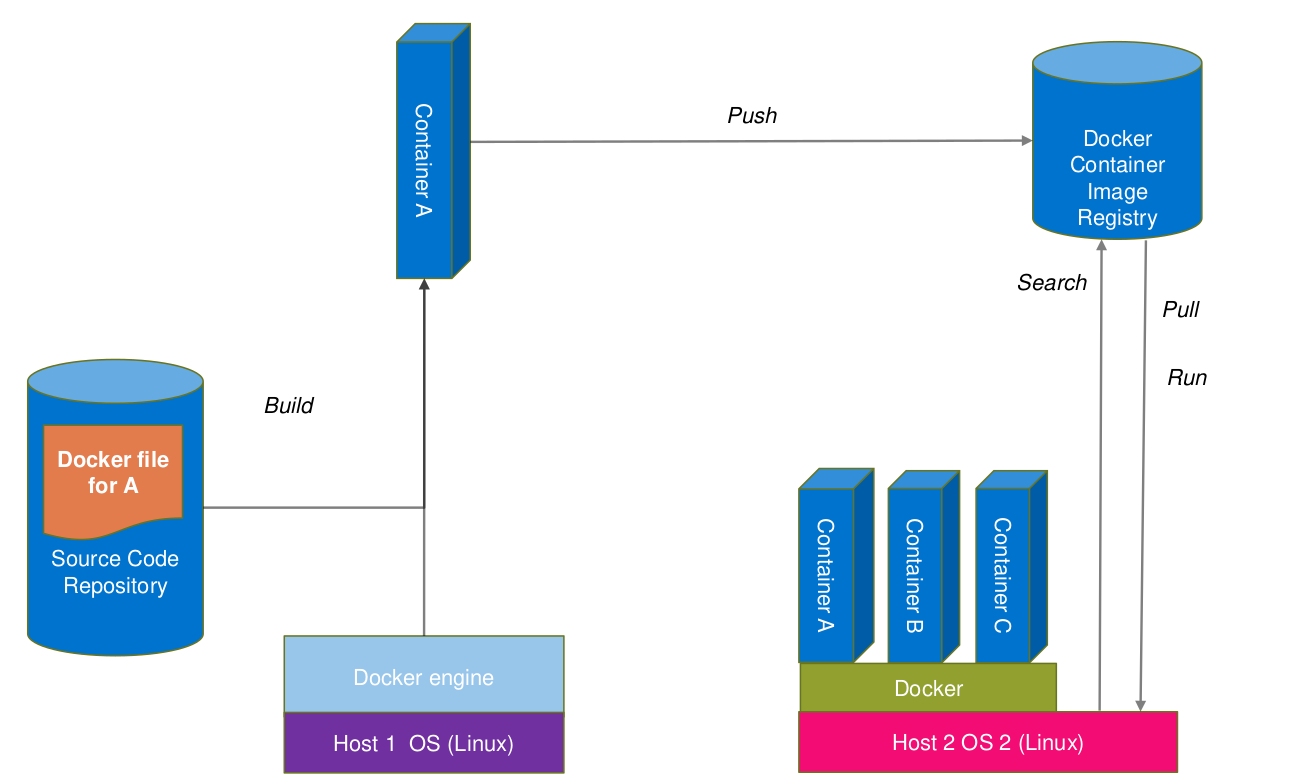
\includegraphics[width=.8\textwidth]{images/docker.png}
  \caption{Docker System}\label{fig:docker}
\end{figure}
